
% \documentclass[fleqn,10pt]{wlscirep}
% fleqn : left alignment of equation

\documentclass[10pt]{wlscirep}
\usepackage[utf8]{inputenc}
\usepackage{amsmath}
\usepackage{amsbsy}
\usepackage[T1]{fontenc}
\usepackage{soul} % 여러 라인에 걸친 밑줄을 사용하기 위한 패키지

\DeclareMathOperator*{\argmin}{arg\,min} % Jan Hlavacek

%from here, code for line numbers
\usepackage{lineno}
\linenumbers

\makeatletter
\patchcmd\@maketitle{%
        {%
        \noindent
        \colorbox{color2}{%
            \parbox{\dimexpr\linewidth-2\fboxsep\relax}{%
            \sffamily\small\textbf\\\theabstract
            }%
        }%
        }%
    }{%
        \nolinenumbers{%
        \noindent
        \colorbox{color2}{%
            \parbox{\dimexpr\linewidth-2\fboxsep\relax}{%
            \internallinenumbers \sffamily\small\theabstract
            }%
        }%
        }%
    }
    {\wlog{true}}{\wlog{false}}
    
\makeatother
%end of code for line numbers

\title{Radionuclide Identification for Plastic Scintillation Detectors by Backward Cumulative Channel Sum}
% \linenumbers
\author[1]{Ji-Yong So}
\author[2]{Byoungil Jeon}
\author[1,*]{Myungkook Moon}
\affil[1]{Korea Atomic Energy Research Institute, Neutron Science Division, Daejeon, 34057, Korea}
\affil[2]{Korea Atomic Energy Research Institute, Applied Artificial Intelligence Section, Daejeon, 34057, Korea}

\affil[*]{moonmk@kaeri.re.kr}

% \affil[+]{These authors equally contributed to this work}

\keywords{radiation portal monitor, radionuclide identification}

\begin{abstract}
Plastic scintillation detectors are widely used in radiation portal monitors (RPMs) due to their low cost, mechanical robustness, and high detection efficiency. However, their inherently poor energy resolution makes radionuclide identification and quantitative analysis challenging, particularly under low-count conditions where spectral features are easily obscured by statistical fluctuations. To address this limitation, we propose a simple and robust spectral-processing framework based on the Backward Cumulative Channel Sum (BCCS) transformation, combined with two complementary background-compensation techniques: direct subtraction and background normalization. The BCCS operation produces smooth, monotonically decreasing cumulative profiles that suppress high-channel noise while preserving essential spectral structure, enabling enhanced separability among radionuclides.
Using reference measurements of Am-241, Cs-137, and Co-60, as well as nine mixed-source configurations acquired under typical RPM conditions, we demonstrate that both background-compensation methods yield processed spectra with improved contrast and distinctive source-dependent signatures. The transformed spectra remain compatible with nonlinear least-squares unfolding, allowing reliable estimation of radionuclide contributions in mixed-source measurements. The estimated contributions exhibit the expected distance-dependent attenuation and remain robust until source activity becomes indistinguishable from background-derived thresholds.
The results show that the proposed BCCS-based framework enables effective radionuclide identification and quantitative activity estimation using only low-resolution plastic scintillation detectors. Because the method is computationally lightweight and requires no specialized hardware or training datasets, it can be readily integrated into existing RPM systems to enhance performance in real operational environments. 
\end{abstract} 

\begin{document}

\flushbottom
\maketitle
% * <john.hammersley@gmail.com> 2015-02-09T12:07:31.197Z:
%
%  Click the title above to edit the author information and abstract
%
\thispagestyle{empty}

% \noindent Please note: Abbreviations should be introduced at the first mention in the main text – no abbreviations lists. Suggested structure of main text (not enforced) is provided below.

\section*{Introduction}

Radiation portal monitors (RPMs) are widely deployed at border crossings, transportation facilities, and industrial sites to detect illicit transportation of radioactive materials\cite{Sicilliano2005Comparision, Bertrand2014Current,Ely2006TheUse}. Most RPM systems utilize large-area plastic scintillation detectors because of their low cost, mechanical robustness, fast response, and high detection efficiency \cite{Hevener2013EWindow, Lee2020Radioisotope, Paff2017Spectral}. However, plastic scintillators inherently exhibit poor energy resolution, and the resulting spectra are dominated by broad Compton continua rather than well-defined photopeaks. This limitation makes radionuclide identification particularly challenging under field conditions, where the net count rate is often low and background radiation can vary significantly over time.

To address these limitations, various signal-processing approaches have been proposed for enhancing spectral discriminability in low-resolution detectors. Traditional techniques include smoothing or denoising filters\cite{Paff2017Spectral}, which aim to suppress statistical noise, and feature-extraction methods based on principal component analysis (PCA)\cite{Runkle2006Analysis,Kim2019InvMat}. More recently, machine-learning and deep-learning approaches have been introduced to improve source classification accuracy using low-resolution gamma-ray spectra\cite{Kim2019ANN,Lee2023Radionuclide,Jeon2021CompML}. While these methods have shown promising results, they often require extensive training datasets or are sensitive to varying measurement conditions, limiting their direct applicability to field-deployed RPM systems. Moreover, approaches relying on computationally intensive inference may not be suitable for embedded systems with strict real-time constraints.

In practical RPM operation, radioactive sources must often be detected at relatively large source-to-detector distances or through shielding, resulting in extremely low net-count measurements. Under such conditions, spectral differences between radionuclides can easily be obscured by background fluctuations. Therefore, a robust preprocessing technique that enhances spectral separability without requiring high-resolution detectors or complex models is highly desirable.

In this work, we propose the Backward Cumulative Channel Sum (BCCS) as an effective spectral transformation for improving radionuclide separability in plastic scintillators. By accumulating counts from high to low channels, the BCCS operation suppresses fluctuations in the high-channel region while preserving meaningful spectral structure. In addition, we investigate two complementary background-compensation schemes—direct subtraction and background normalization—to isolate source-specific contributions under low-count conditions.

The transformed and background-compensated spectra retain linearity, enabling quantitative spectral decomposition using nonlinear least-squares unfolding. Through experimental measurements of Am-241, Cs-137, and Co-60, including multiple mixed-source configurations at various source-to-detector distances, we demonstrate that the proposed methods support both qualitative radionuclide identification and quantitative activity estimation using only low-resolution plastic scintillation detectors.

\section*{Methods}
\subsection*{Experimental Setup}
Gamma-ray spectra were measured using a large-volume plastic scintillator (30 cm $\times$ 180 cm $\times$ 5 cm) coupled to a photomultiplier tube and a multichannel analyzer with 2048 channels. Three radionuclides—Am-241, Cs-137, and Co-60—were used as reference sources, and each spectrum was measured together with an independently acquired background spectrum at multiple source-to-detector distances. To evaluate mixed-source scenarios, nine combinations of the three radionuclides were also measured at varying distances. All measurements were conducted under typical radiation portal monitoring conditions, with acquisition times selected to reflect practical low-count environments.

The raw spectra exhibit broad Compton continua with most counts concentrated in the low-energy region, as expected for plastic scintillation detectors. These spectra form the basis for subsequent preprocessing, background compensation, and quantitative analysis.

\subsection*{Spectral Preprocessing: Backward Cumulative Channel Sum (BCCS)}

Let

$$
\mathbf{C} = [C_1,\,C_2,\ldots,\,C_N]
$$

denote a raw pulse-height spectrum where $C_i$ is the count in channel $i$.The Backward Cumulative Channel Sum (BCCS) is defined as

\begin{equation}
B_i = \sum_{j=i}^N C_j. \label{eq:BCCS}
\end{equation}

Unlike the conventional forward cumulative spectrum that sums from the first channel upward, the BCCS accumulates counts from channel 
$i$ to the end of the spectrum. This produces a smooth, monotonically decreasing cumulative profile that suppresses statistical fluctuations in the high-channel region while preserving the global spectral structure. Because this transform enhances separability under low-count conditions, it serves as the primary preprocessing step for all subsequent analyses.


\subsection*{Background Compensation Techniques}

Two complementary background-compensation methods were applied after BCCS transformation: direct subtraction and normalization to background.

\subsubsection*{(a) Direct Subtraction Method}

Let $\mathbf{B}^X$ and $\mathbf{B}^\textrm{bkg}$ denote the BCCS spectra of source $X$ and background, respectively. The background subtracted spectrum $\mathbf{S}^X = [S^X_1,\ldots,S^X_N]$ is then defined as

\begin{equation}
S^X_i =  B^X_i - B_i^{\textrm{bkg}}. \label{eq:DS}
\end{equation}

This operation preserves the count scale and yields an interpretable representation of the source contribution. Due to statistical fluctuations, small negative values may appear—most notably for Am-241, whose spectrum is concentrated in the lowest channels. These negative values are less than one-tenth of the maximum amplitude and arise purely from noise; therefore, they are set to zero during the unfolding process to avoid spurious effects.

%Owing to the cumulative nature of BCCS, negative values rarely occur even for weak signals, making the method inherently robust against over-subtraction.

\subsubsection*{(b) Normalization to Background Method} 

To emphasize relative deviations from background, each BCCS spectrum is normalized by the background distribution. Therefore, the normalized spectrum $\mathbf{R}^X=[R^X_1,\ldots,\,R^X_N]$ is defineds as

\begin{equation}
R^X_i = \left(\dfrac{B^X_i}{B^{\textrm{bkg}}_i}\right) -1=\dfrac{S^X_i}{B_i^{\text{bkg}}}.\label{eq:NB}
\end{equation}

The resulting dimensionless profile highlights local spectral contrast while suppressing global count-level variations. This method is particularly effective when the source signal only slightly exceeds background, enabling reliable pattern recognition in low-count conditions.

These two methods provide complementary perspectives—absolute (subtraction) and relative (normalization)—and ensure robust performance under diverse measurement scenarios.

\subsection*{Radionuclide Activity Estimation via Linear Spectral Unfolding}

The contribution of each radionuclide in a measured spectrum $\mathbf{C}^M=[C_1,\ldots,\,C_N]$ is estimated using nonlinear least-squares spectral unfolding. After applying same BCCS and one of background compensation process for the measured spectrum and its background $\mathbf{C}^{M,\,\text{bkg}}$, we have $\mathbf{S}^M$ or $\mathbf{R}^M$. For direrct subtranction method, we can model the measured spectrum as a linear combination of reference spectra, such as :

\begin{equation}
S_i^M = \sum_X \alpha_X S_i^X,\label{eq:submethod}
\end{equation}

\noindent where $\alpha_X$ denotes its contribution. Because meaningful spectral features are present only in the lower channels for plastic scintillators under low-count conditions, the unfolding is performed over the restricted channel range Similary, for the ratio-normalized spectra, we obtain

\begin{equation*}
R_i^M = \sum_X \alpha_X \left(\dfrac{S_i^X}{B_i^{M,\text{bkg}}}\right).
\end{equation*}

If the background distributions of the measured spectrum and reference spectra are compareble, i.e., $B^{M,\text{bkg}}_i \approx B_i^{X,\text{bkg}}$, then

\begin{equation}
R_i^M = \sum_X \alpha_X \left(\dfrac{S_i^X}{B_i^{X,\text{bkg}}}\right) = \sum_X \alpha_X R_i^X.\label{eq:ratiomethod}
\end{equation}

In both cases-direct subtraction (\ref{eq:submethod}) and ratio normalizaiton (\ref{eq:ratiomethod})-the coefficients $\alpha_X$ can be estimated by solving the non-negative least squares (NNLS) problem :

\begin{equation}
\argmin_{\alpha_X \ge 0} \left\| \textbf{I}^{\text{M}} - \sum_{X} \alpha_X \textbf{I}^{X}\right\|^2,\label{eqn:llns}
\end{equation}

where $\bf{I}^M$ and $\bf{I}^{X}$ denote the measured and reference spectra after applying the chosen background compensation method.

This procedures provide physically meaningful, non-negative estimates of radionuclide contributions, even in the presence of spectral overlap, low counts, or poor energy resolutions. By appying NNLS to both direct-subtraction spectra dn ratio-normalized spectra, reliable decomposition of mixed-source measurements can be achieved.

\section*{Results}

%Up to three levels of \textbf{subheading} are permitted. Subheadings should not be numbered.

\subsection*{Spectral Transformation of Reference Radionuclides Spectra}

Figure \ref{fig:bkgref}(a) shows the raw spectra of background radiation and three reference radionuclides—Am-241, Cs-137, and Co-60—measured using a large-volume plastic scintillator. As expected for plastic scintillation detectors, all spectra are dominated by broad Compton continua, with most counts concentrated in the low-energy region. Cs-137 and Co-60 exhibit noticeable deviations from background over a wide channel range, while Am-241 differs only in the lowest channels, making identification challenging under low-count conditions.

Application of the BCCS transformation yields smooth, monotonically decreasing profiles, as shown in Figure \ref{fig:bkgref}(b). This operation suppresses statistical fluctuations in the high-channel region and enhances spectral separability. Figures \ref{fig:bkgref} (c) and \ref{fig:bkgref} (d) respectively present the background-subtracted and background-normalized BCCS spectra. The subtraction method retains absolute count information, while normalization emphasizes relative deviations. Both provide improved visibility of radionuclide-specific features compared to the raw spectra.


\subsection*{Background Compensation }

% **OLD**

% Two background compensation methods—direct subtraction and normalizaiton to backgorund—were applied to the BCCS-transformed spectra to improve separation between background and source contributions. The direct subtraction method effectively isolated the net source signal by removing the background BCCS spectrum, producing interpretable cumulative profiles that preserved radionuclide-specific spectral characteristics (Figure \ref{fig:bkgref} (c)). This behavior remained consistent in mixed-source measurements, where the resulting spectra maintained mixture-dependent features that reflect the relative contributions of individual radionuclides (Figure \ref{fig:mixedbccs} (a)). 

% In the case of Am-241, the spectrum is concentrated almost entirely in the very low-channel region. As a result, statistical fluctuations can generate small negative values in the background-subtracted BCCS spectrum. These negative values are less than one-tenth of the maximum amplitude of the Am-241 signal and therefore contribute negligibly to the overall spectral shape. Since they arise purely from statistical noise rather than any physical process, they are set to zero in the subsequent fitting procedure to prevent spurious effects in the quantitative analysis. 

% The ratio-based normalization method (Figure \ref{fig:bkgref} (d)) emphasized proportional deviations from the background spectrum, revealing characteristic source-induced patterns even under low-count conditions. By suppressing global count-level variations, this method enhanced the visibility of subtle spectral differences and improved pattern recognition when source signals only slightly exceeded background levels.

% Together, these two approaches provide complementary perspectives: direct subtraction captures absolute source contributions, while ratio normalization highlights relative contrasts. Their combined use supports robust spectral interpretation across a wide range of measurement scenarios, including low-count and mixed-source environments.


% **NEW**

Mixed-source spectra were processed using the same two background-compensation methods. Figure \ref{fig:mixedbccs} (a) shows the mixed-source BCCS spectra obtained with direct subtraction, and Figure \ref{fig:mixedbccs} (b) presents the corresponding normalize to background spectra. The normalized representation provides enhanced visual contrast, particularly when radionuclides produce distinct Compton features in different channel regions or when the overall count rate is relatively high. Under these conditions, mixed-source compositions become more readily distinguishable, supporting clear qualitative interpretation prior to quantitative analysis.

Due to the strong low-channel concentration of Am-241, statistical fluctuations may produce small negative values after subtraction. These values are less than one-tenth of the Am-241 peak amplitude and arise purely from noise; thus, they are set to zero during the unfolding process to avoid distortions in the fitting.




\subsection*{Spectral unfolding and Radioisotope identification}

Figure \ref{fig:mixedbccs}(a) presents the mixed-source spectra obtained using the background-subtracted BCCS method, while Figure \ref{fig:mixedbccs}(b) shows the corresponding results produced by background normalization. A comparison of the two approaches indicates that the background-normalized spectra provide a more intuitive visual representation of source presence, particularly when the overall radiation intensity is relatively high or when the constituent radionuclides contain Compton features in different channel regions. In such cases, the ratio-normalized spectra accentuate these differences more distinctly, enabling mixed-source compositions to be recognized more readily. This enhanced visual contrast also facilitates subsequent quantitative decomposition through linear spectral unfolding.

Applying nonlinear least-squares fitting to Eq. \ref{eqn:llns} enables estimation of the contribution of each radionuclide for both background-compensation methods. Due to the low net counts and the absence of distinctive spectral features in the high-channel region, only the low-channel range ($0 \le i \le 100$) is used for the fitting. Figures \ref{fig:fi_fitbgsub} and \ref{fig:fi_fitbgrto} present the fitting results for the background-subtracted and background-normalized spectra, respectively, each illustrating the estimated contributions of the reference radionuclides.

Figure \ref{fig:fi_fitcontrib} summarizes the estimated contributions as a function of source-to-detector distance. The horizontal dashed lines indicate the mean contributions obtained from samples that do not contain the corresponding radionuclide. The monotonic decrease in contribution with increasing distance aligns with general expectations based on geometric attenuation. As observed for Co-60 and Cs-137, when the activity of a radionuclide becomes sufficiently low, its contribution can no longer be reliably determined using this method. These results demonstrate that the proposed data-processing techniques enable effective radionuclide identification and quantitative activity estimation for plastic scintillation detectors.

\subsection*{Summary of Results}

Overall, the proposed preprocessing, background compensation, and unfolding framework provides clear separation of radionuclide signatures, even in low-count mixed-source scenarios.

\begin{itemize}
    \item BCCS transformation enhances spectral smoothness and separability.
    \item Direct subtraction and background normalization offer complementary perspectives, improving qualitative interpretation.
    \item Nonlinear spectral unfolding enables reliable quantitative estimation of radionuclide activities across multiple configurations.
\end{itemize}

These results demonstrate that effective radionuclide identification and activity estimation can be achieved using low-resolution plastic scintillation detectors without requiring additional hardware or high-resolution spectroscopy systems.

\section*{Discussion}

The results presented in this study demonstrate that the proposed BCCS-based preprocessing framework, combined with direct subtraction or background normalization, provides a robust approach for enhancing radionuclide identification and quantitative analysis using plastic scintillation detectors. Although plastic scintillators inherently lack the energy resolution required to resolve photopeaks, the BCCS transformation effectively suppresses high-channel statistical fluctuations while preserving the essential spectral tendencies of different radionuclides. This greatly enhances the separability of spectral patterns under low-count conditions, which represent the most challenging operational regime for radiation portal monitors.
A notable advantage of the proposed approach is its simplicity and compatibility with real-time processing. Unlike machine-learning or data-driven methods that require extensive training datasets and may generalize poorly to new environments, the BCCS transformation and background-compensation procedures operate directly on measured spectra without prior training. This ensures stable performance even when background levels fluctuate or when measurement conditions vary across deployments. The cumulative nature of BCCS also mitigates the effect of individual spectral bins with large Poisson fluctuations, enabling more consistent interpretation of weak-source signals.

Direct subtraction and background normalization play complementary roles in isolating source contributions. Subtraction provides absolute information, which is useful for quantifying net source intensity, while normalization enhances relative contrast and highlights spectral deviations that are otherwise difficult to observe. Their combined use ensures robustness across a wide range of operational scenarios. For example, normalization yields clearer identification in mixed-source configurations where radionuclides exhibit Compton features in distinct channel regions. In contrast, subtraction retains physically meaningful count scales, enabling accurate nonlinear least-squares unfolding for quantitative activity estimation.
The unfolding results further demonstrate that reliable radionuclide contribution estimates can be obtained up to moderate distances, beyond which contributions fall below the background-derived thresholds. This behavior reflects fundamental physical limitations—geometric attenuation and statistical noise—rather than limitations of the processing method itself. Indeed, the proposed approach identifies and quantifies radionuclides down to the point where their activity becomes indistinguishable from background, indicating that the technique is operating near the practical detection limit for plastic scintillators. The use of a restricted low-channel fitting range($0\le i \le 100$) was found to be effective for minimizing noise-induced artifacts while preserving sufficient information for accurate unfolding.

The methods evaluated in this work are particularly relevant for field-deployed RPM systems, where low-cost, high-efficiency detectors are favored over high-resolution but more fragile alternatives such as HPGe. The proposed framework requires no specialized hardware and can be implemented on existing RPM platforms with minimal computational overhead, making it suitable for embedded real-time analysis. Moreover, the generality of the approach suggests applicability to other low-resolution detection environments where background compensation and weak-signal enhancement are critical, including drone-based radiation surveys, portable screening devices, and wide-area monitoring systems.

Despite its advantages, several limitations remain. The accuracy of unfolding depends on the quality and stability of reference spectra, and deviations due to environmental changes or detector aging may introduce biases. In addition, the current implementation assumes that background spectra are measured under conditions comparable to those of source measurements. Future work may consider adaptive background modeling, temporal background estimation, or Bayesian unfolding frameworks to incorporate uncertainties more systematically. Extending the approach to include additional radionuclides or shielding scenarios may also improve general applicability.

Overall, the findings of this study indicate that the combination of BCCS preprocessing, background compensation, and nonlinear spectral unfolding provides a practical and effective solution for radionuclide identification and activity estimation using low-resolution plastic scintillation detectors. The methods improve both qualitative interpretability and quantitative performance, suggesting strong potential for enhancing next-generation RPM systems without requiring modifications to detector hardware.

\section*{Conclusion}

In this study, we developed and evaluated a spectral-analysis framework for improving radionuclide identification and activity estimation using low-resolution plastic scintillation detectors. The proposed method combines the Backward Cumulative Channel Sum (BCCS) transformation with two complementary background-compensation techniques—direct subtraction and background normalization—to enhance spectral separability under low-count conditions typical of radiation portal monitoring applications.
The BCCS transformation effectively suppresses statistical fluctuations in the high-channel region while preserving essential spectral structure. When paired with background subtraction or normalization, the processed spectra exhibit improved contrast and source-specific signatures that are more readily distinguishable than those in raw spectra. Furthermore, the transformed spectra remain compatible with nonlinear least-squares spectral unfolding, enabling quantitative estimation of radionuclide contributions in mixed-source measurements.

Experimental results obtained using Am-241, Cs-137, and Co-60—across multiple source-to-detector distances and mixed compositions—demonstrate that the proposed approach achieves reliable source identification and activity estimation without requiring high-resolution detectors or data-intensive training procedures. The results indicate that the method remains robust until the underlying source activity becomes indistinguishable from background levels, reflecting the fundamental detection limits of plastic scintillators.

Because the approach is computationally lightweight and does not require hardware modifications, it can be readily integrated into existing RPM systems or other field-deployable radiation detection platforms. Future work will focus on extending the method to broader source sets, incorporating adaptive background modeling, and evaluating performance under dynamic or moving-source scenarios.

Overall, the proposed BCCS-based framework offers a practical and effective solution for enhancing the performance of plastic scintillator–based radiation portal monitors, supporting both qualitative radionuclide identification and quantitative activity analysis in real operational environments.

\section*{Acknowledgements}

This research was supported by the Ministry of Oceans and Fisheries, Korea, through the Korea Institute of Marine Science \& Technology Promotion (KIMST) under Project No. 20200611. The authors acknowledge the use of ChatGPT (OpenAI) for language refinement and editorial assistance during the preparation of this manuscript. All scientific content, interpretations, and conclusions presented herein were solely developed and validated by the authors.

\section*{Author contributions statement}
M. Moon conceived the study and performed the experiments. J. So developed the analysis software and performed signal processing. B. Jeon synthesized the test datasets and supported evaluation. All authors contributed to writing and reviewing the manuscript.

\bibliography{./biblio}

\section*{Additional information}

% To include, in this order: \textbf{Accession codes} (where applicable); \textbf{Competing interests} (mandatory statement). 

% The corresponding author is responsible for submitting a \href{http://www.nature.com/srep/policies/index.html#competing}{competing interests statement} on behalf of all authors of the paper. This statement must be included in the submitted article file.


\begin{figure}[ht]
\centering
% 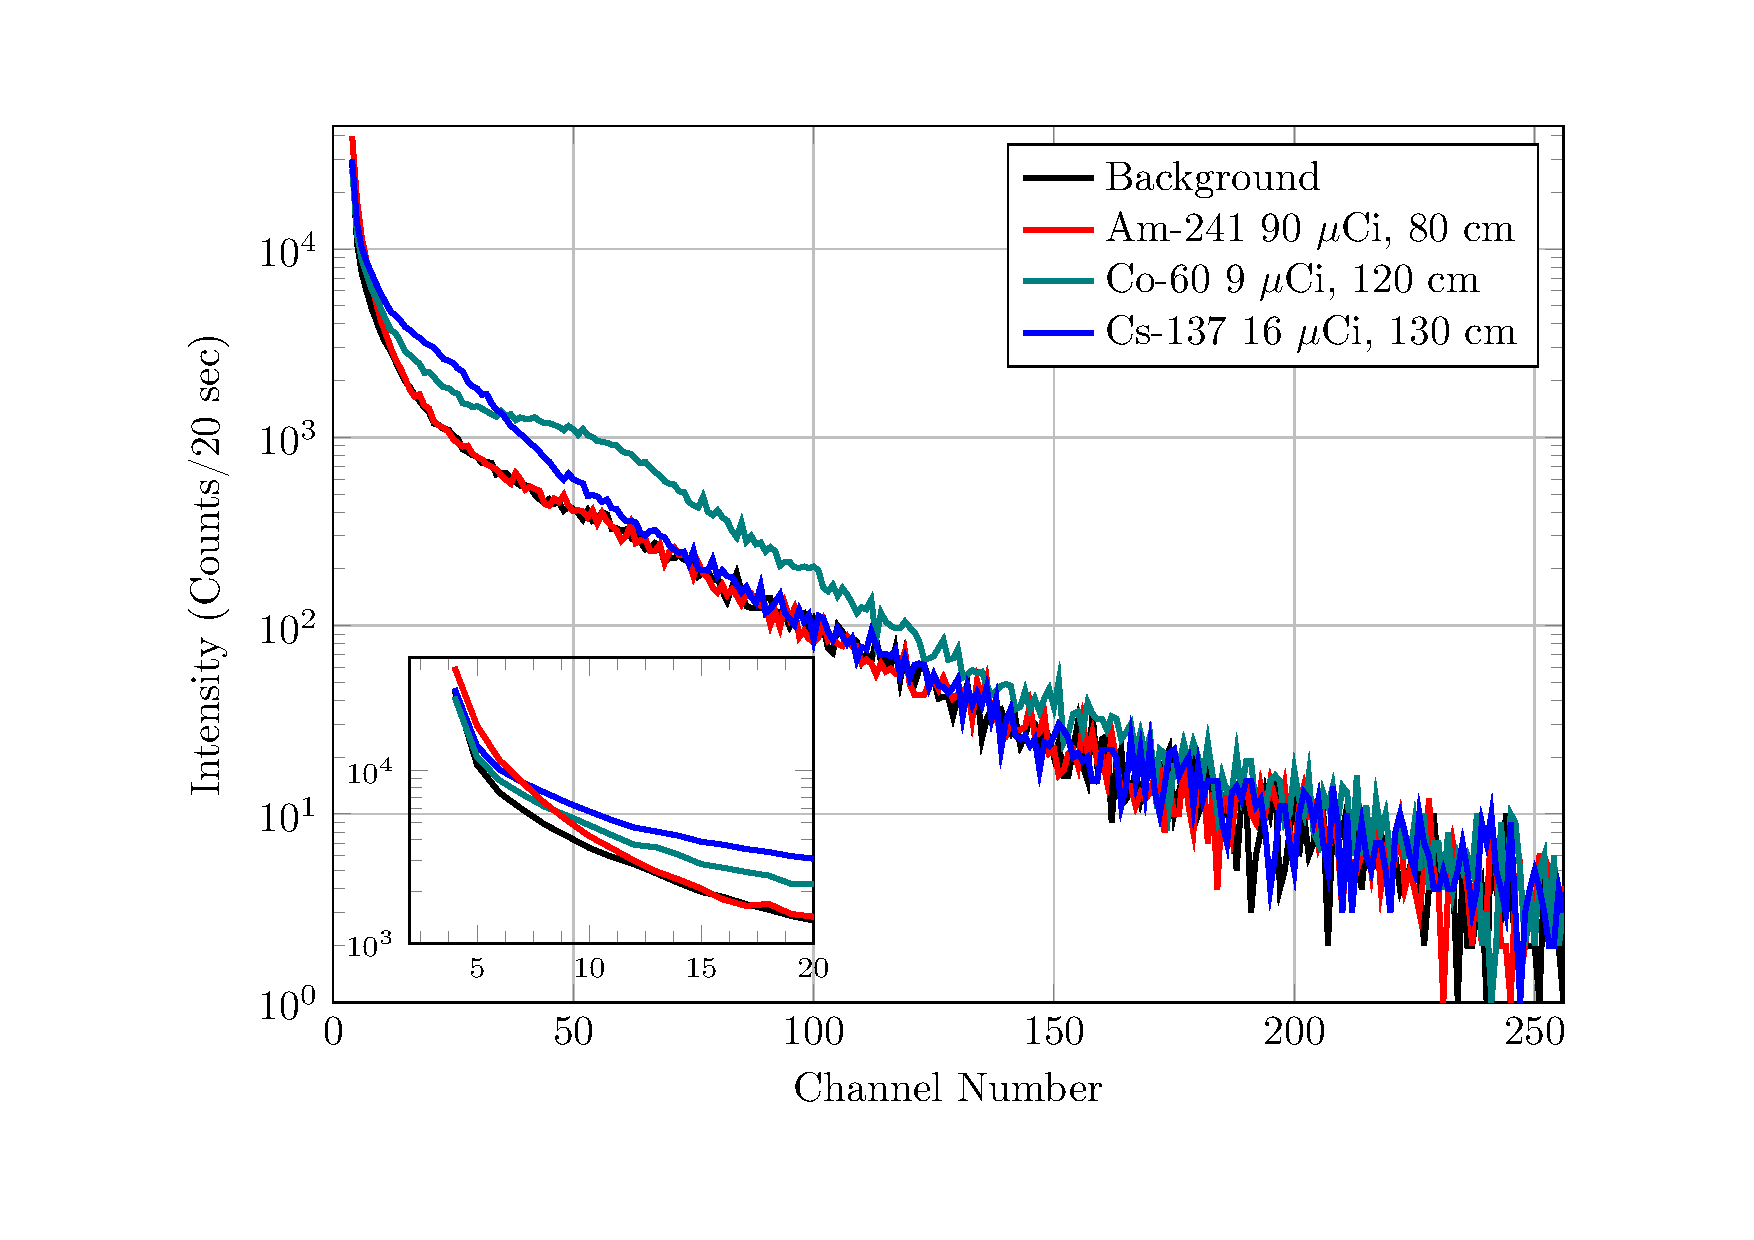
\includegraphics[width=\linewidth]{figure/fig01_bkgref.pdf}
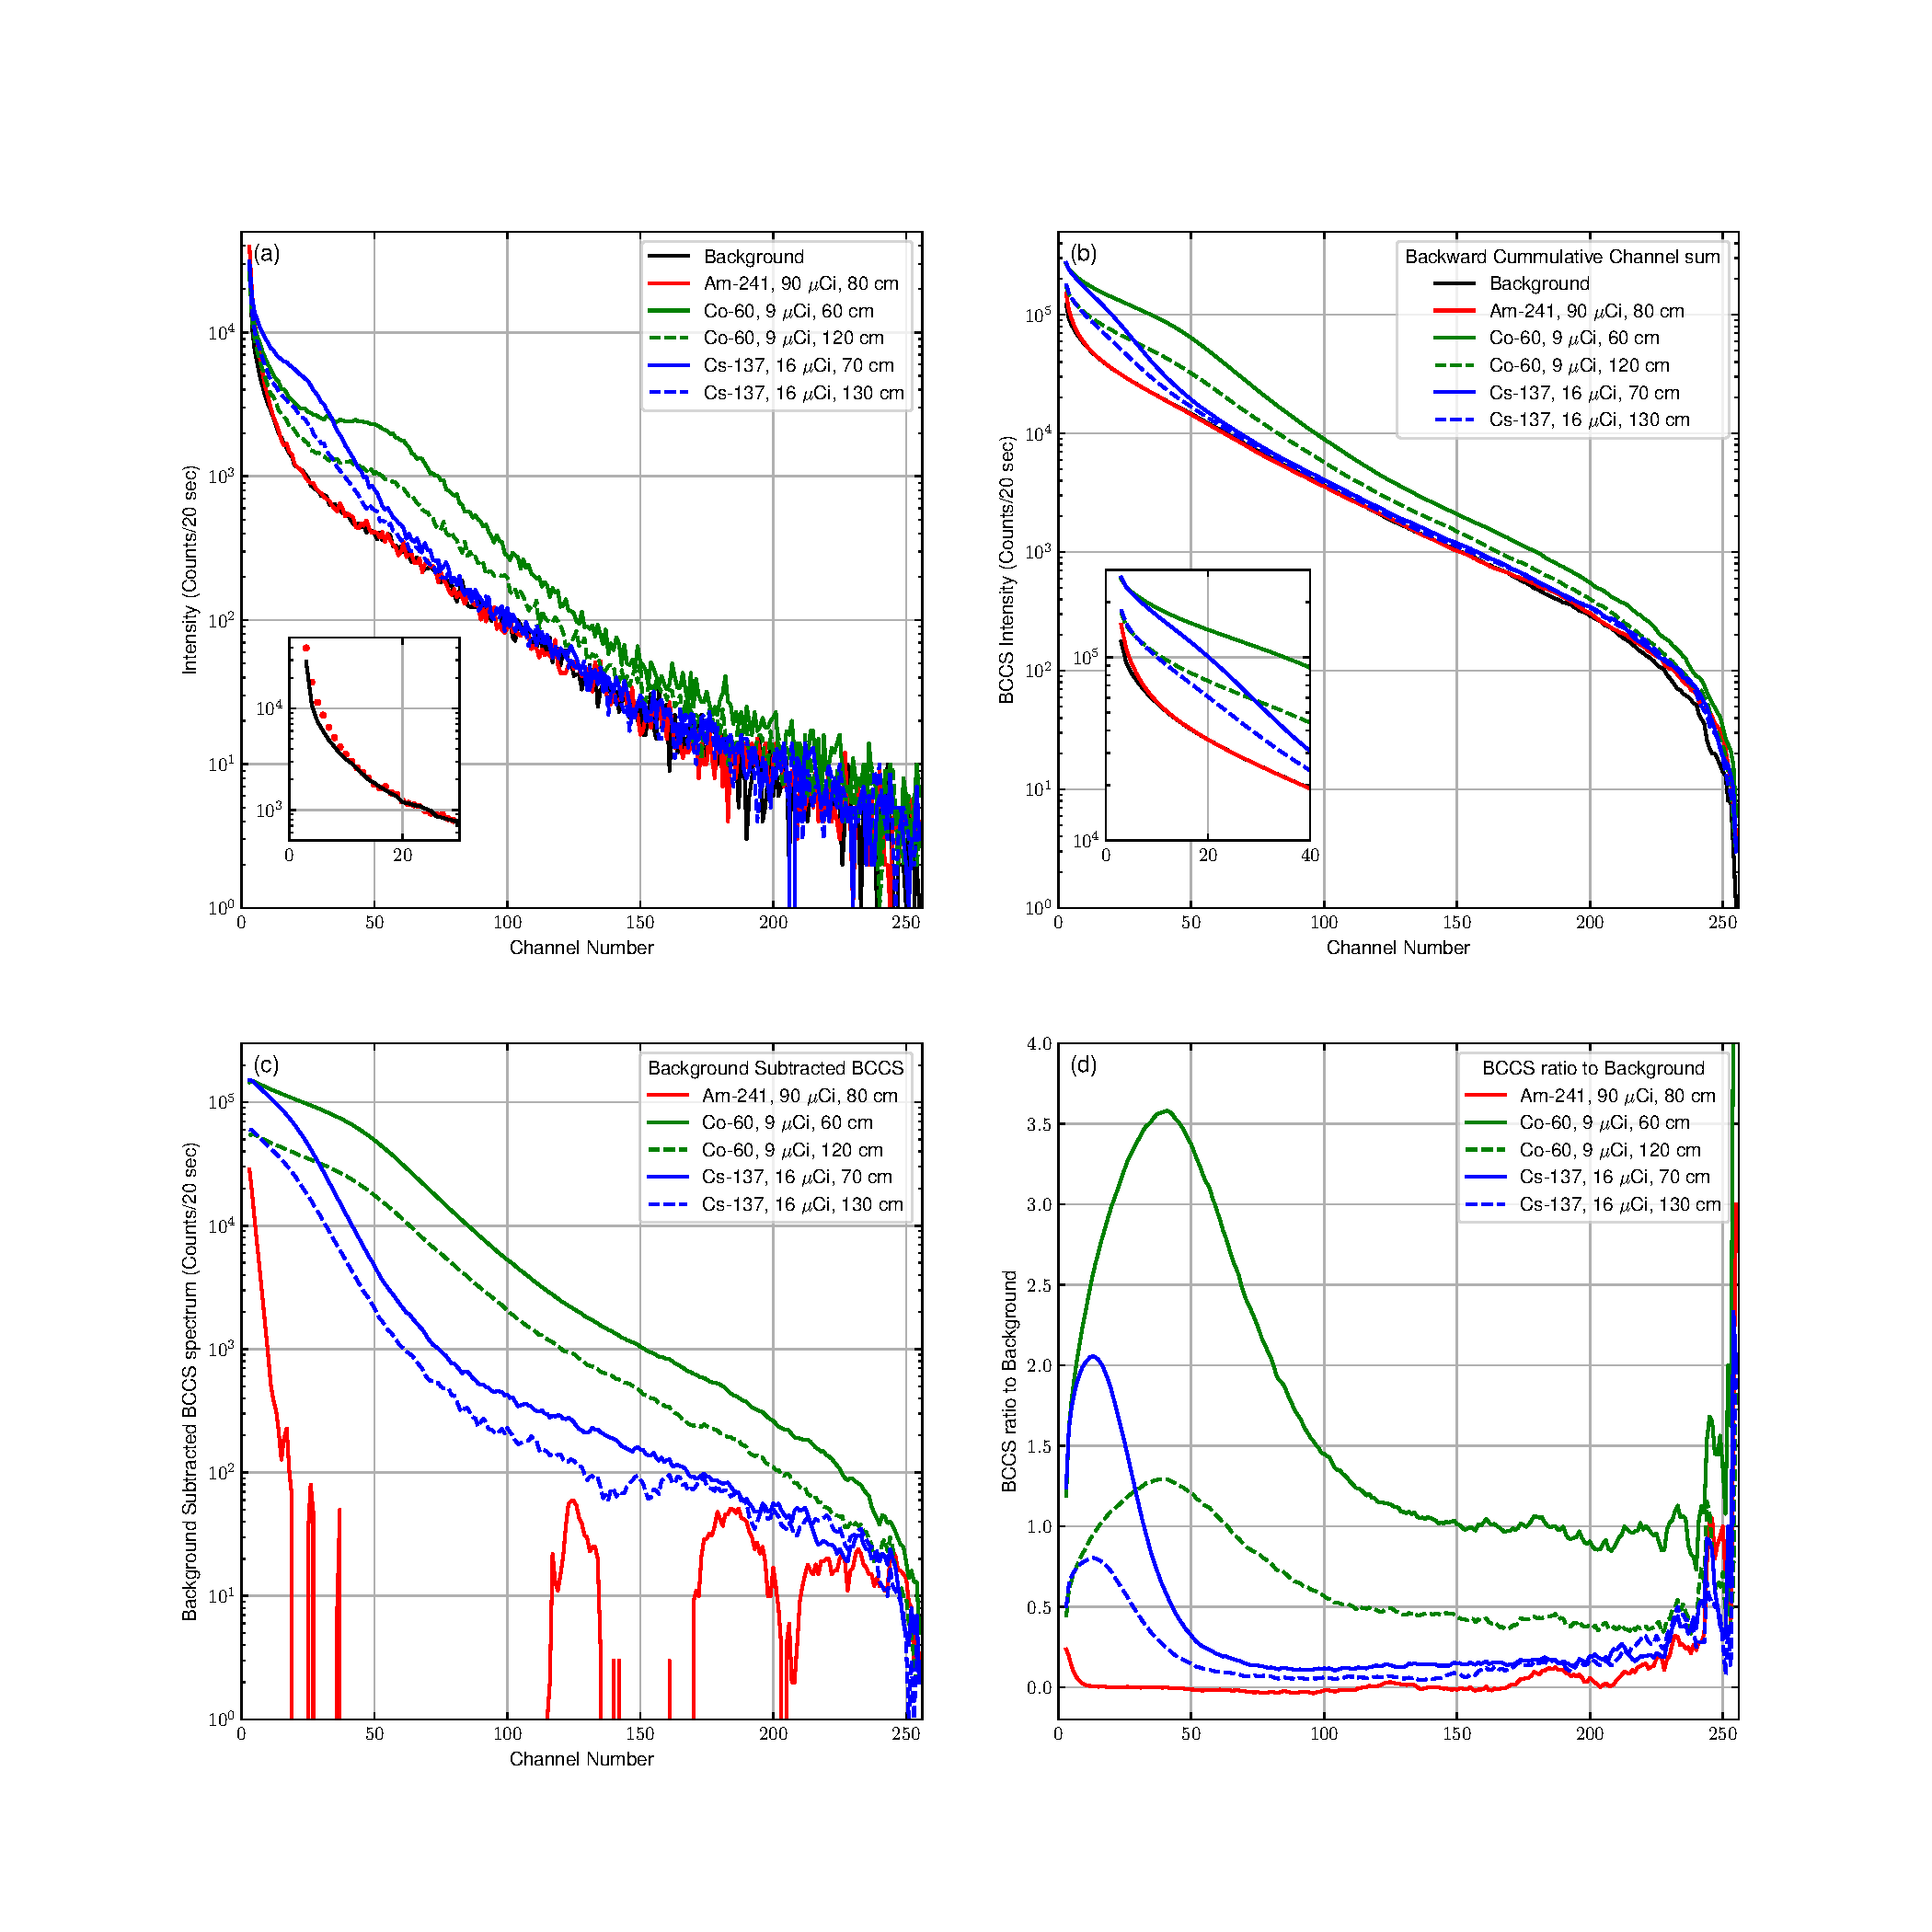
\includegraphics[width=\linewidth]{newfigures/figure1.pdf}
\caption{(a) Raw gamma-ray spectra of background radiation and three reference radionuclides (Am-241, Cs-137, and Co-60) measured using a large-volume plastic scintillation detector. As typical for plastic scintillators, all spectra are dominated by broad Compton continua, with most counts concentrated in the low-channel region.
(b) Corresponding BCCS-transformed spectra, showing smooth, monotonically decreasing profiles that suppress high-channel statistical fluctuations while preserving overall spectral structure.
(c) Background-subtracted BCCS spectra, which reveal source-specific deviations from background while retaining the count scale.
(d) Background-normalized BCCS spectra, highlighting relative intensity differences and enhancing visual contrast under low-count conditions.}

\label{fig:bkgref}
\end{figure}

\newpage 

\begin{figure}[ht]
\centering
% 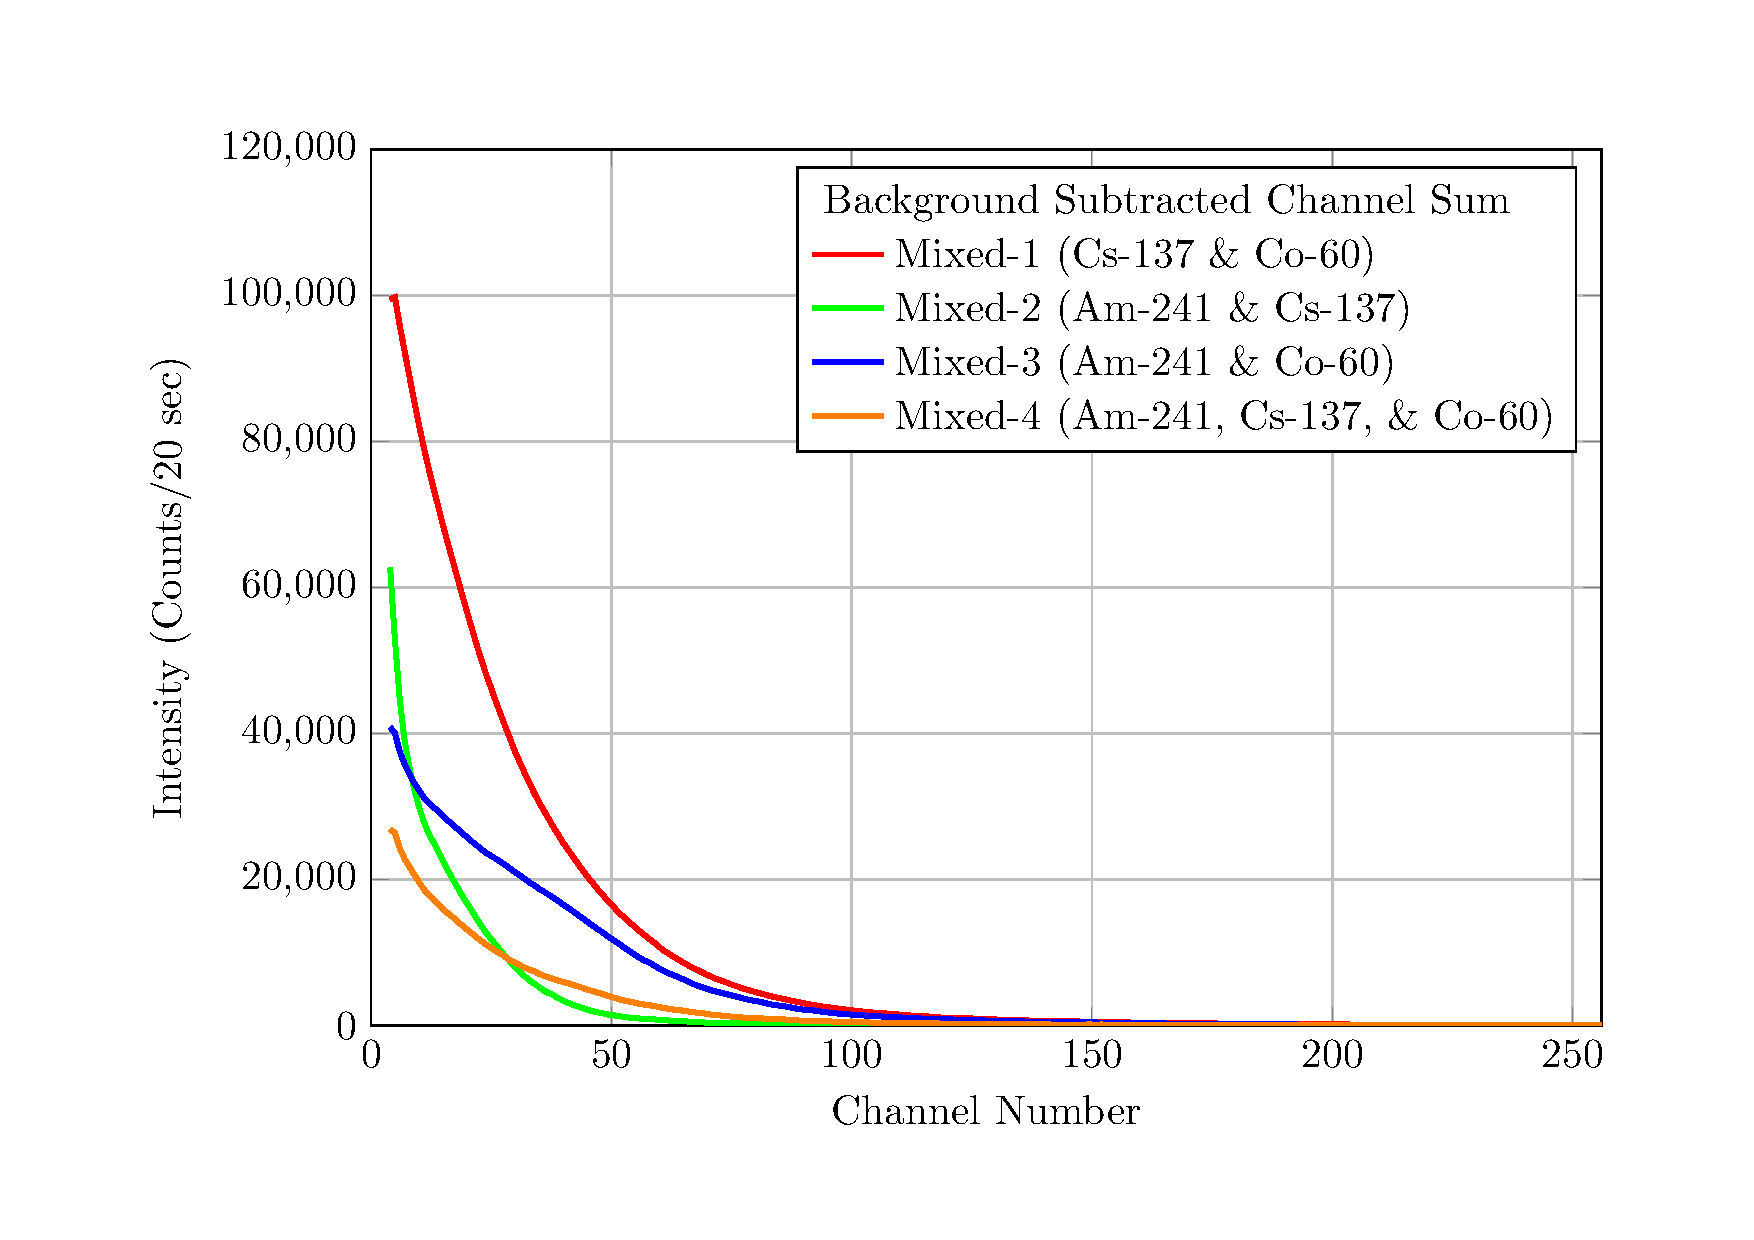
\includegraphics[width=\linewidth]{figure/fig04_CSBS.pdf}
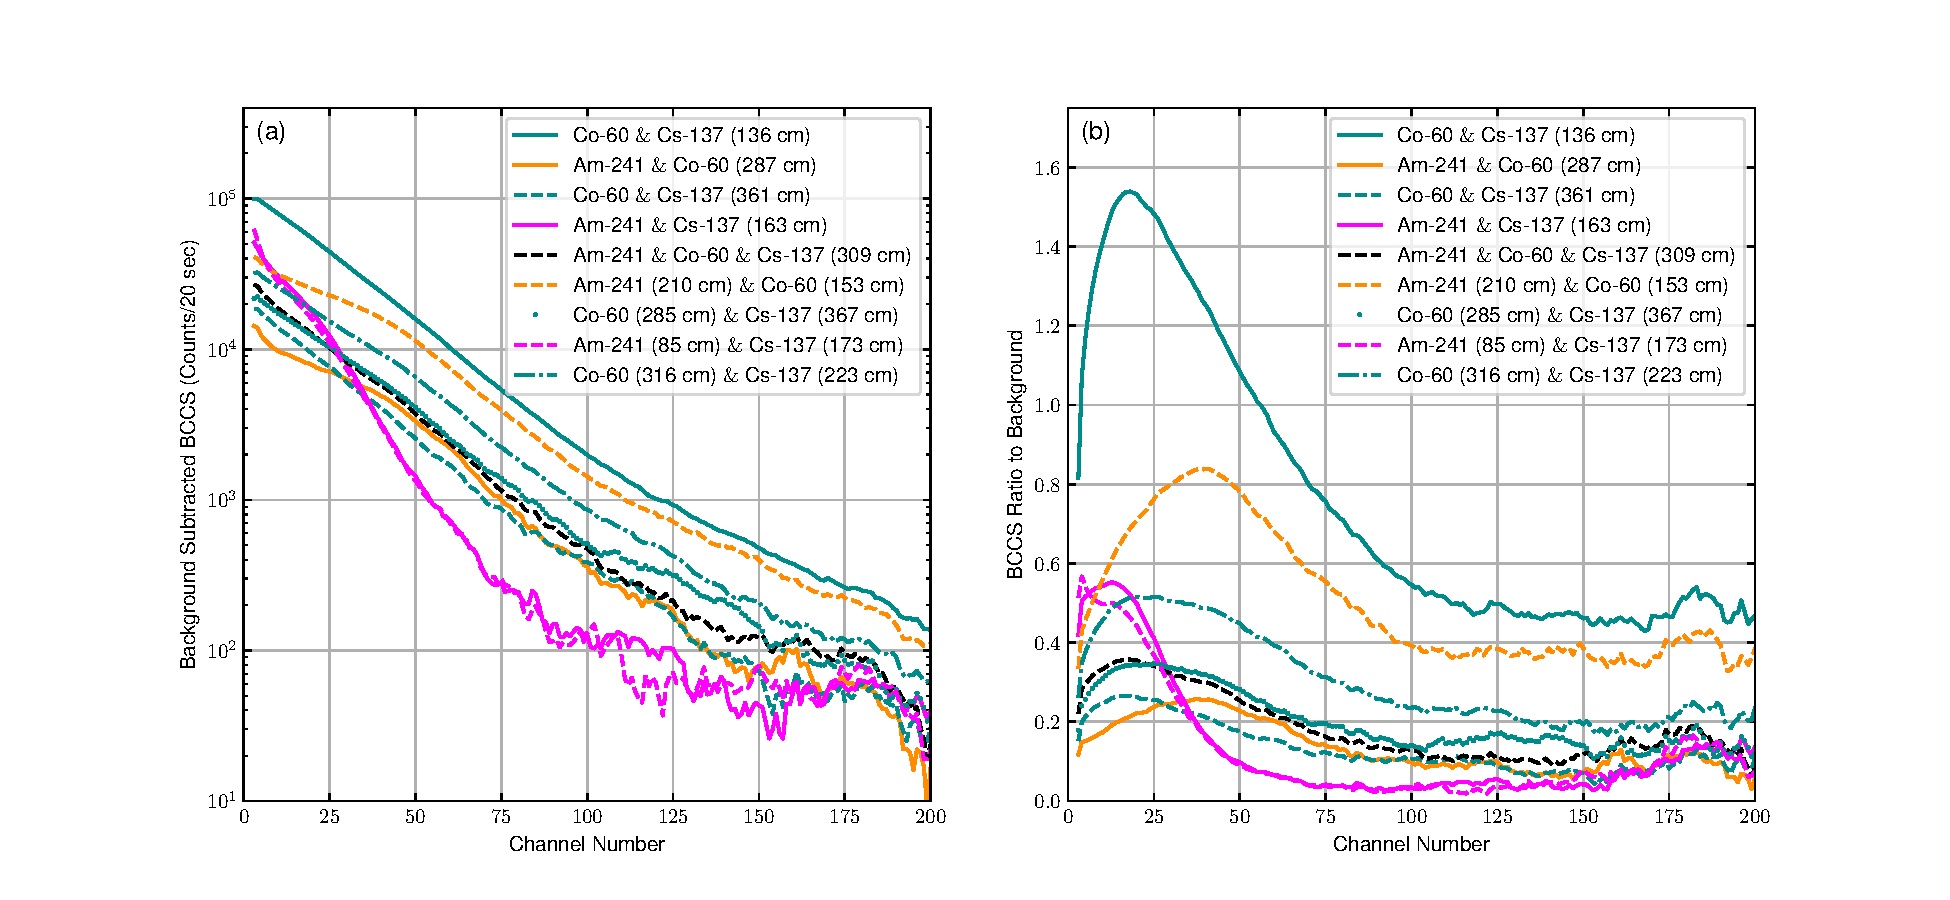
\includegraphics[width=\linewidth]{newfigures/figure2.pdf}
\caption{(a) Background-subtracted BCCS spectra for nine mixed-source configurations consisting of Am-241, Cs-137, and Co-60 at various source-to-detector distances. Absolute count differences among mixtures are preserved, revealing mixture-dependent cumulative spectral profiles.
(b) Background-normalized BCCS spectra for the same configurations. Normalization emphasizes relative deviations from background and enhances the visibility of spectral differences among mixtures, particularly when radionuclides exhibit distinct Compton features in different channel regions.}
\label{fig:mixedbccs}
\end{figure}

\newpage


\begin{figure}[ht]
\centering
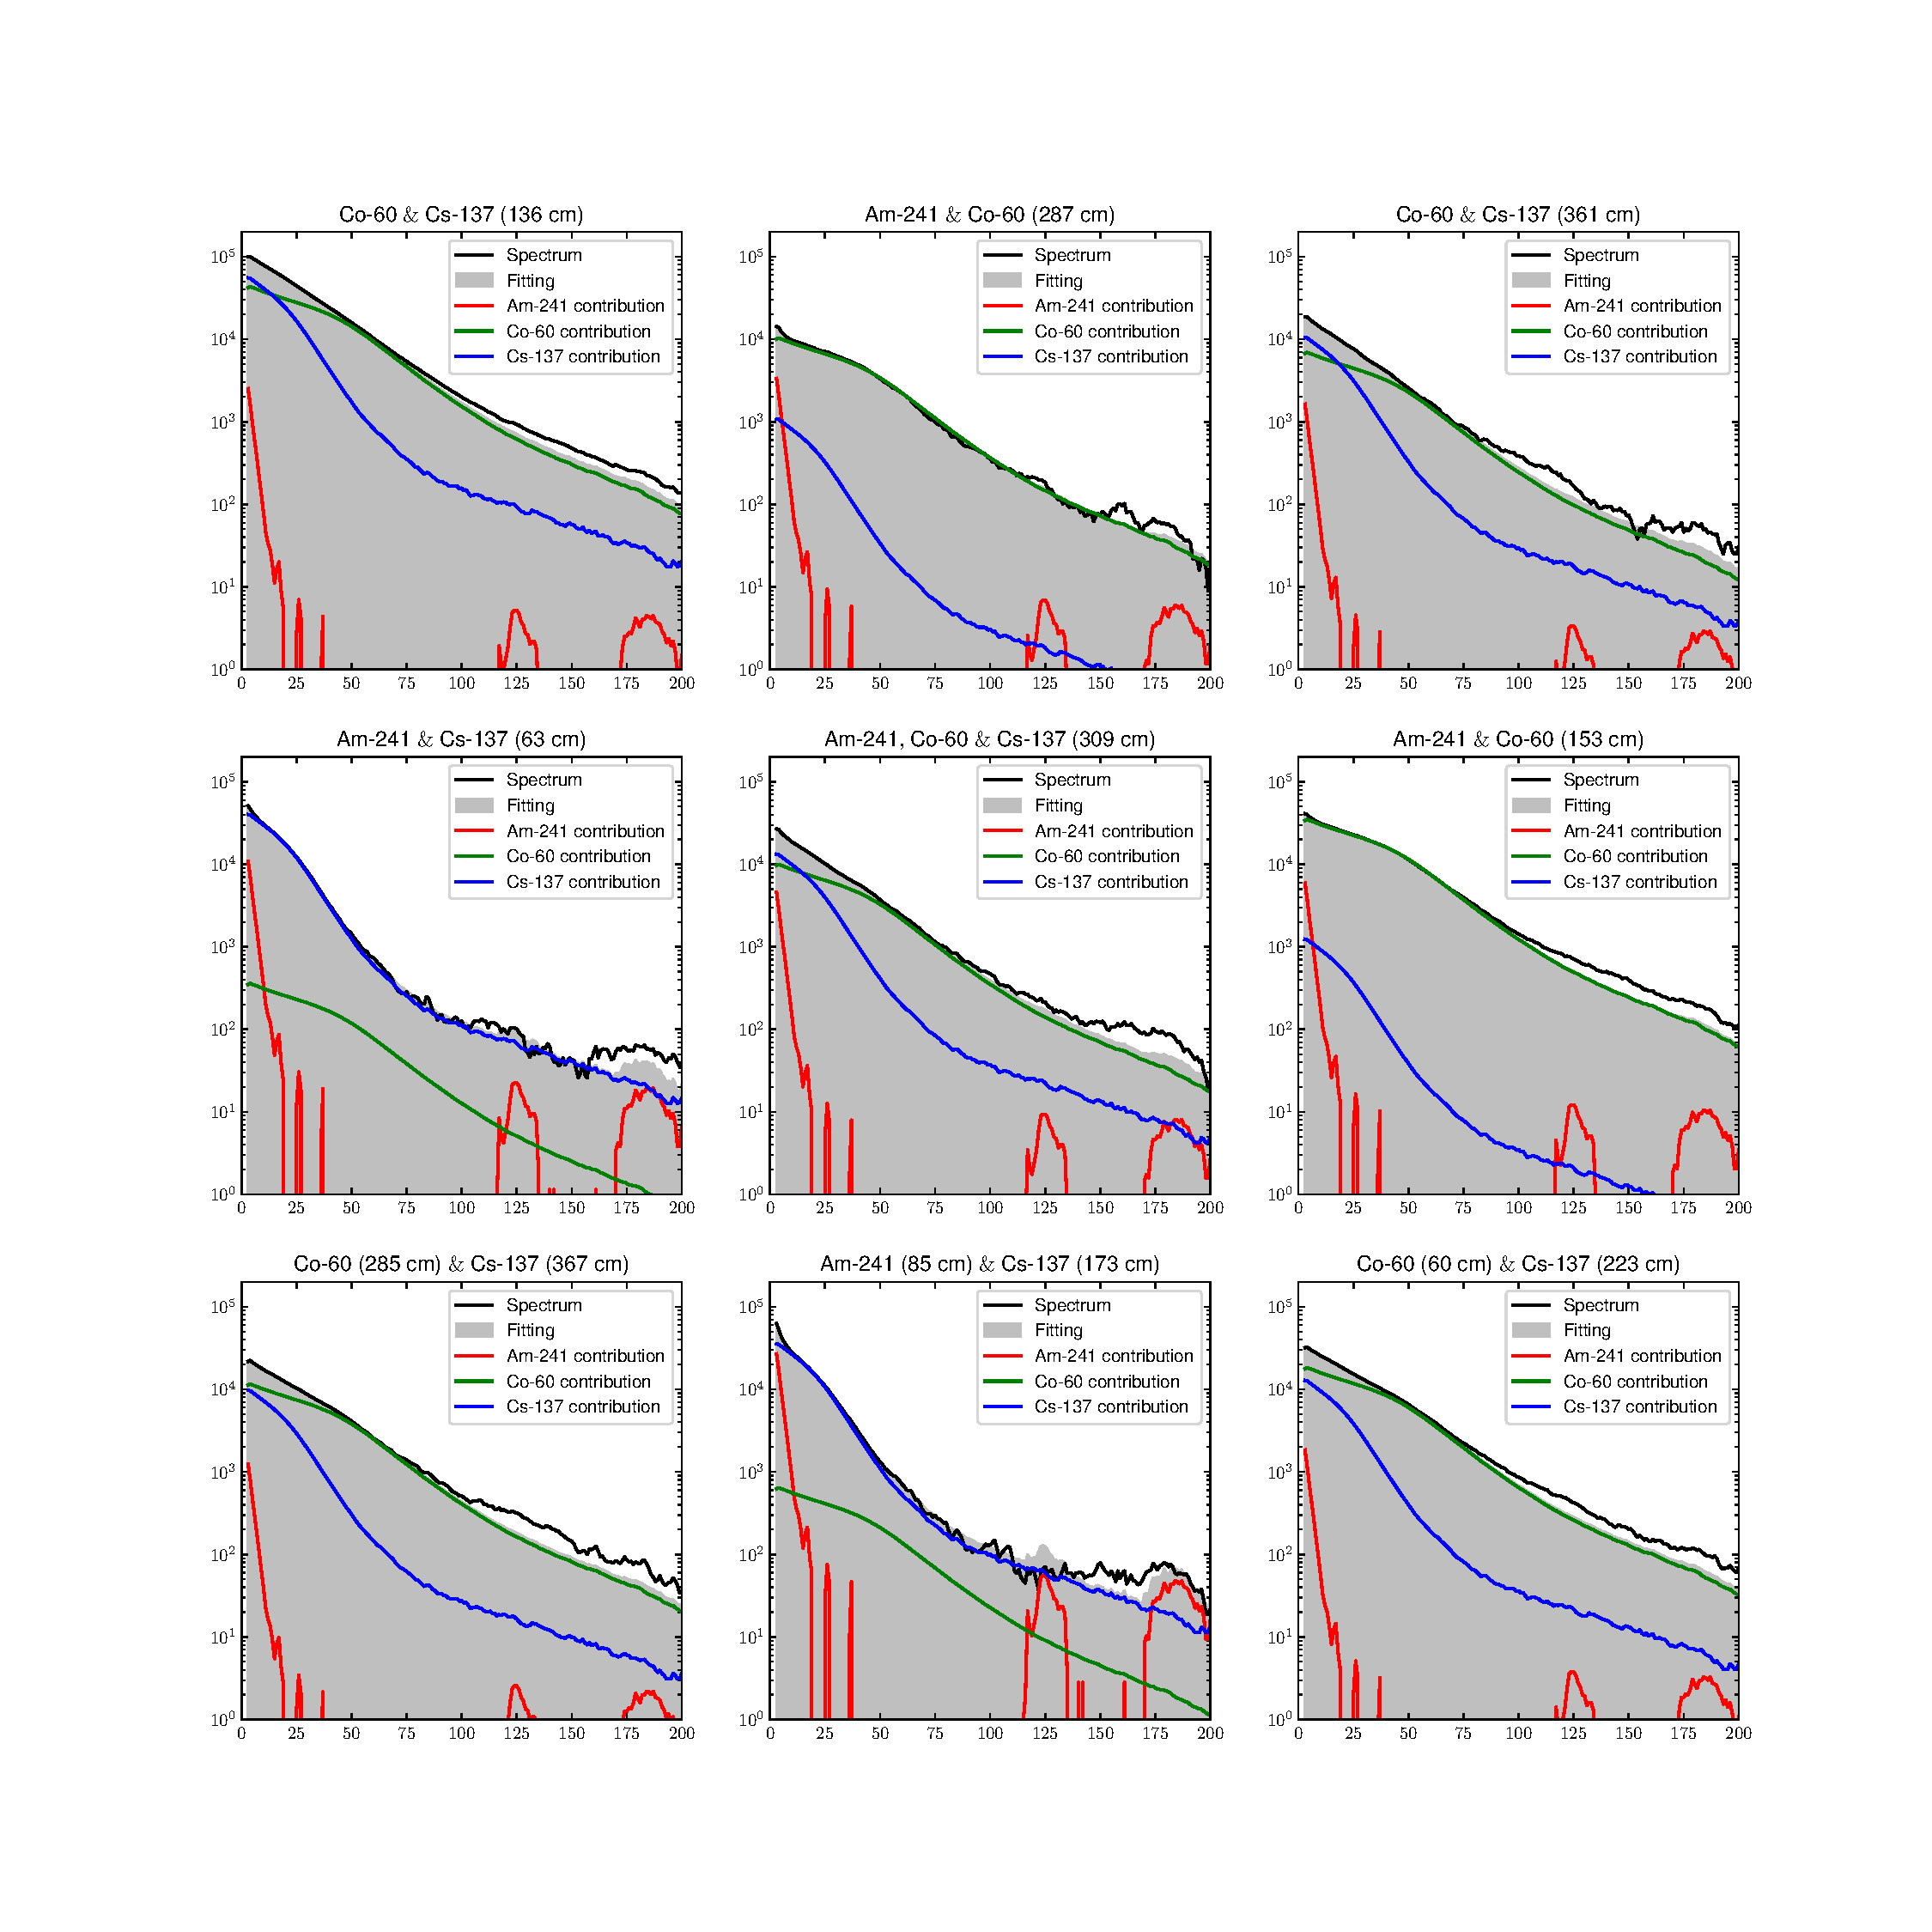
\includegraphics[width=\linewidth]{figure/fit_BGSub.pdf}
\caption{Nonlinear least-squares fitting results for the background-subtracted BCCS spectra of the nine mixed-source configurations. Each panel shows the measured background-subtracted spectrum (black) together with the fitted spectrum obtained from the linear combination of reference radionuclides (colored). The inferred contribution coefficients ($\alpha_\text{Am-241},\, \alpha_\text{Cs-137},\, \alpha_\text{Co-60}$) for each mixture are shown in the legend. The close agreement between the measured and reconstructed spectra demonstrates that the unfolding based on background-subtracted BCCS profiles provides reliable decomposition of mixed-source measurements under low-count conditions.}
\label{fig:fi_fitbgsub}
\end{figure}

\begin{figure}[ht]
\centering

\includegraphics[width=\linewidth]{newfigures/fit_BGRto.pdf}
\caption{Nonlinear least-squares fitting results for the background-subtracted BCCS spectra of the nine mixed-source configurations. Each panel shows the measured background-subtracted spectrum (black) together with the fitted spectrum obtained from the linear combination of reference radionuclides (colored). The inferred contribution coefficients ($\alpha_\text{Am-241},\, \alpha_\text{Cs-137},\, \alpha_\text{Co-60}$) for each mixture are shown in the legend. The close agreement between the measured and reconstructed spectra demonstrates that the unfolding based on background-subtracted BCCS profiles provides reliable decomposition of mixed-source measurements under low-count conditions.}
\label{fig:fi_fitbgrto}
\end{figure}

\begin{figure}[ht]
\centering
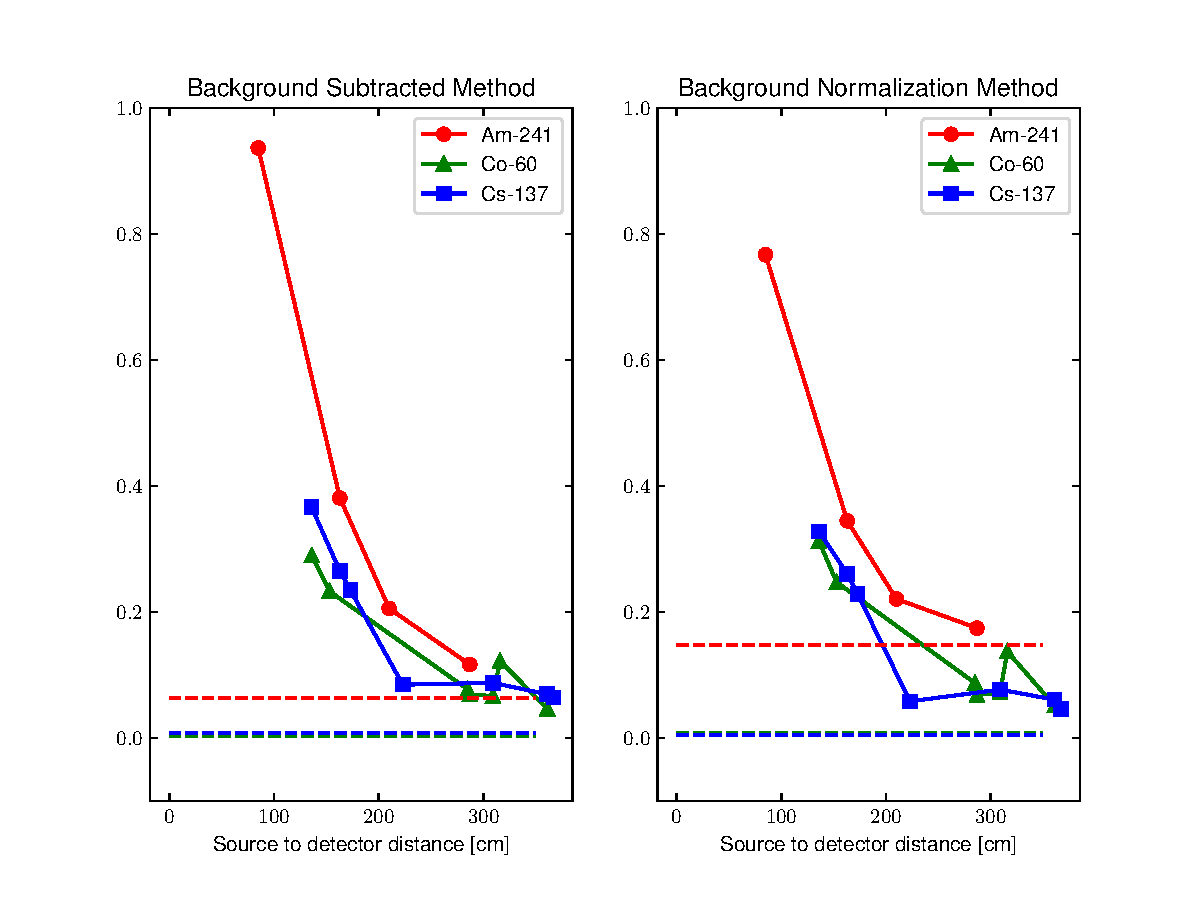
\includegraphics[width=\linewidth]{newfigures/fit_contributions.pdf}
\caption{Estimated radionuclide contributions ($\alpha_\text{Am-241},\, \alpha_\text{Cs-137},\, \alpha_\text{Co-60}$)  as a function of source-to-detector distance, obtained from nonlinear spectral unfolding using the processed BCCS spectra. The horizontal dashed lines represent the mean contributions estimated from measurements in which the corresponding radionuclide is absent, serving as effective decision thresholds. The contributions decrease monotonically with increasing distance, consistent with geometric attenuation. For Co-60 and Cs-137, the estimated contributions converge to their respective threshold bands at large distances, indicating that the activity is no longer distinguishable from background under such low-count conditions.}
\label{fig:fi_fitcontrib}
\end{figure}

\end{document}